%%=============================================================================
%% Methodologie
%%=============================================================================

\chapter{Methodologie}
\label{ch:methodologie}

%% TODO: Hoe ben je te werk gegaan? Verdeel je onderzoek in grote fasen, en
%% licht in elke fase toe welke stappen je gevolgd hebt. Verantwoord waarom je
%% op deze manier te werk gegaan bent. Je moet kunnen aantonen dat je de best
%% mogelijke manier toegepast hebt om een antwoord te vinden op de
%% onderzoeksvraag.

Om een antwoord te vinden op de vastgelegde onderzoeksvragen dient er natuurlijk een experiment uitgevoerd te worden. Hoe dit experiment opgesteld wordt zal hieronder nader verklaart worden.

\section{Plan van aanpak}
Het experiment zal uitgevoerd worden op enkele testpersonen die momenteel een kinesist raadplegen voor een letsel aan de bovenste ledematen. De bedoeling is dat de patiënt samen met de kinesist eerst enkele oefeningen uitvoert zonder de hulp van VR. Hierover krijgt hij dan een vragenlijst en dient zaken in te vullen zoals: hoe was de pijnervaring tijdens de oefeningen?, bent u altijd even gemotiveerd om uw oefeningen uit te voeren?, etc. Daarna zal de patiënt de VR bril opgezet krijgen en aan de hand van de ontwikkelde applicatie en de hulp van de kinesist de oefeningen nogmaals uitvoeren. De kinesist kan de bewegingen van de patiënt meevolgen op het computerscherm om verdere intructies te verschaffen. Wanneer de kinesist dit wenst zijn er ook polsgewichten ter beschikking om de oefeningen wat uitdagender te maken voor de patiënt. Aan het einde van de oefensessie met VR zal de patiënt opnieuw een vragenlijst dienen in te vullen.


\chapter{Experiment}

\section{Materiaal}
Om het experiment uit te voeren zijn er enkele zaken nodig van materiaal:

- VR headset en controller: Hier wordt de Oculus Go gebruikt

- Computer: Hierop worden de vragenlijsten ingevuld na de oefensessies. Ook zal de kinesist hierop kunnen zien wat de patiënt in het spel aan het doen is.

- Polsgewichten: Deze kunnen bij de patiënt omgedaan worden om de intensiteit van de oefeningen te vergroten.


\subsection{Testpersonen}
Voorlopig nog fake testpersonen (voor draft)

\section{Resultaten}

\begin{figure}[h]
    \centering
    \includegraphics[scale=0.8]{chart_PijnZonderVR.png}
    \caption{Pijnervaring van testpersonen zonder gebruik van VR}
\end{figure}

\begin{figure}[h]
    \centering
    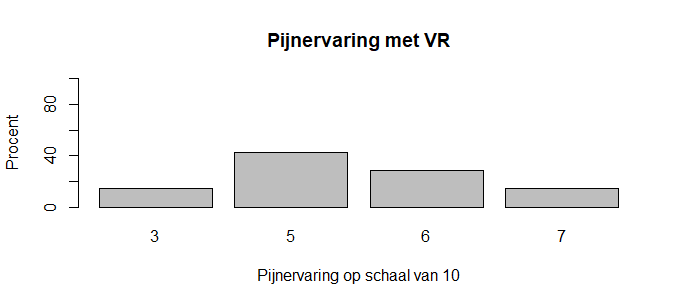
\includegraphics[scale=0.8]{chart_pijnMetVR.png}
    \caption{Pijnervaring van testpersonen met gebruik van VR}
\end{figure}



